\documentclass[MTech]{iitmdiss}
\usepackage{times}
\usepackage{epsf}
\usepackage{threeparttable}
\usepackage{setspace}
\usepackage{amsmath}
\usepackage{bm}
\usepackage{amsthm}
\usepackage{txfonts,pxfonts,amsfonts}
\usepackage{epsfig}	
\usepackage{caption}

%\usepackage{subfigure}
%\usepackage{subcaption}
%\usepackage[english]{babel}
%\usepackage[utf8]{inputenc}
%\usepackage[nottoc]{tocbibind}
%\usepackage{subtable}
%\usepackage{subcaption}
\usepackage{listings}
\usepackage{epstopdf}

%\usepackage[dvips]{graphicx}
\usepackage{graphicx,subfigure}
\usepackage{comment}
%\usepackage{pstricks,pst-node,pst-tree,pstricks-add}
\usepackage[square,numbers,sort]{natbib}
%\usepackage{biblatex}
%\usepackage[square]{natbib}
\usepackage{hyperref}
%\usepackage[hypertex]{hyperref} % hyperlinks for references.
%\usepackage{algorithmic}
%\usepackage{algorithm}

\usepackage[ruled]{algorithm2e}% http://ctan.org/pkg/algorithm2e
\makeatletter
\renewcommand{\@algocf@capt@plain}{above}% formerly {bottom}
\makeatother

\newcommand\blfootnote[1]{%
  \begingroup
  \renewcommand\thefootnote{}\footnote{#1}%
  \addtocounter{footnote}{-1}%
  \endgroup
}
%\include{commands}

% Strut macros for skipping spaces above and below text in tables. 
\def\abovestrut#1{\rule[0in]{0in}{#1}\ignorespaces}
\def\belowstrut#1{\rule[-#1]{0in}{#1}\ignorespaces}

\def\abovespace{\abovestrut{0.20in }}
\def\aroundspace{\abovestrut{0.20in}\belowstrut{0.10in}}
\def\belowspace{\belowstrut{0.10in}}
%%%%%%%%%%%%%%%%%%%%%%%%%
\def\thesistitle{OPTIMIZING COMPUTATION OF BETWEENNESS CENTRALITY IN GRAPHS}
\def\thesisauthor{TEJAS SHAH}

\begin{document}
\bibliographystyle{iitm}
%%%%%%%%%%%%%%%%%%%%%%%%%%%%%%%%%%%%%%%%%%%%%%%%%%%%%%%%%%%%%%%%%%%%%% 
% Title page

\title{\thesistitle}
\author{\thesisauthor}
%\guide{Rupesh Nasre}
\date{November 2017}
\department{Computer Science and Engineering}

%\nocite{*}
\begin{singlespace}
\maketitle 
\end{singlespace} 



%%%%%%%%%%%%%%%%%%%%%%%%%%%%%%%%%%%%%%%%%%%%%%%%%%%%%%%%%%%%%%%%%%%%%%
% Certificate
\certificate
\vspace*{0.5in}
\noindent This is to certify that the thesis entitled {\bf {\thesistitle}}, 
submitted by {\bf {\thesisauthor}}, Roll no \textbf{CS16M026}, to the Indian Institute of Technology, 
Madras, for the award of the degree of {\bf Master of Technology}, 
is a bonafide record of the research work carried out by her under my
supervision. The contents of this thesis, in full or in parts, have not been
submitted to any other Institute or University for the award of any degree or diploma.
\vspace*{1.4in}
\hspace*{-0.25in}
\begin{singlespace}
\noindent {\bf Prof.~Rupesh~Nasre} \\
\noindent Research Guide \\ 
\noindent Professor \\
\noindent Dept. of Computer Science and Engineering\\
\noindent IIT-Madras, 600 036 \\
\end{singlespace}
\vspace*{0.20in}
\noindent Place: Chennai\\ 
Date: 9 September 2017


%%%%%%%%%%%%%%%%%%%%%%%%%%%%%%%%%%%%%%%%%%%%%%%%%%%%%%%%%%%%%%%%%%%%%%
% Acknowledgements
\acknowledgements
My foremost gratitude and respects to my guide Dr. Rupesh Nasre for his guidance, motivation and moral support in my execution of this project work. His passionate talks about the subject and the many hour-long discussions renewed the zeal in me to keep trying despite the unsatisfying results. His patience with students has been incredible.

I thank Somesh Singh and other PACE lab students for lending their immense help in my work. 

I thank all my classmates and seniors in IITM for their presence that made life happy and incredible here. Their inputs have been significant in every step of these two years.

I thank my parents for being highly accommodating of my erratic schedules and for their love and support. I thank God for making all of this happen.
%%%%%%%%%%%%%%%%%%%%%%%%%%%%%%%%%%%%%%%%%%%%%%%%%%%%%%%%%%%%%%%%%%%%%%

%%%%%%%%%%%%%%%%%%%%%%%%%%%%%%%%%%%%%%%%%%%%%%%%%%%%%%%%%%%%%%%%%%%%%%
% Abstract
\abstract

\noindent KEYWORDS: \hspace*{0.5em} \parbox[t]{4.4in}{Betweenneess Centrality, Graph, BFS, APSP, SSSP}

\vspace*{24pt}

The betweenness centrality index is essential in the analysis of social networks, but costly to compute. Currently, the fastest known algorithm requires $O(n*m)$ time and $O(n+m)$ space, where $n$ is the number of actors in the network and $m$ is total number of connections amongst them which are unweighted. The existing  Brandes' algorithm does all pairs shortest path and calculates centrality. New algorithms for betweenness of a graph are introduced which tried to improvise the execution time using the same time complexity but failed to do so with respect to existing best available algorithm. However, time complexity has been improved for Trees whereas some execution time improvisation has been achieved for DAGs also.
\pagebreak
%%%%%%%%%%%%%%%%%%%%%%%%%%%%%%%%%%%%%%%%%%%%%%%%%%%%%%%%%%%%%%%%%
% Table of contents etc.
\begin{singlespace}
\tableofcontents
\thispagestyle{empty}
\listoftables
\addcontentsline{toc}{chapter}{LIST OF TABLES}
\listoffigures
\addcontentsline{toc}{chapter}{LIST OF FIGURES}
\end{singlespace}
%%%%%%%%%%%%%%%%%%%%%%%%%%%%%%%%%%%%%%%%%%%%%%%%%%%%%%%%%%%%%%%%%%%%%%
% Abbreviations
\abbreviations
\noindent 
\begin{tabbing}
xxxxxxxxxxx \= xxxxxxxxxxxxxxxxxxxxxxxxxxxxxxxxxxxxxxxxxxxxxxxx \kill

\textbf{BC} \> Betweenness Centrality \\
\textbf{APSP} \> All Pairs Shortest Path \\
\textbf{SSSP} \> Single Source Shortest Path \\
\textbf{BFS} \> Breadth First Search \\
\textbf{DFS} \> Depth First Search \\


\end{tabbing}
 
\pagenumbering{arabic}
%%%%%%%%%%%%%%%%%%%%%%%%%%%%%%%%%%%%%%%%%%%%%%%%%%
 % Chapters.
\chapter{INTRODUCTION}
\label{chap:intro}
\section{Overview}

In social network analysis, graph-theoretic concepts are used to understand and explain social phenomena. A social network consists of actors which may or may not share a relation amongst them. An important metric for the analysis of social networks are centrality which are based on the vertices of the graph. The centrality metric ranks the actors of the network according to their importance in the social structure \cite{doi:10.1080/0022250X.2001.9990249}. One such centrality is betweenness.

In graph theory, betweenness centrality in a graph is a metric based on shortest paths. For each pair of vertices in a connected graph, there exists at least one shortest path between them. This shortest path is determined by the fact that for unweighted graphs, the number of edges that the path passes through is minimized and for weighted graphs, the sum of the weights of the edges is minimized. So for a vertex $v$, the betweenness centrality $bc[v]$ is sum of ratio of the number of shortest paths between any pair of vertices $s$ and $t$, other than vertex $v$ which passes through $v$ and total number of shortest paths between $s$ and $t$ \cite{10.2307/3033543}.
The betweenness centrality of a vertex $v$ is given by the expression:

\begin{equation} \label{eqstart}
bc[v] = \sum_{s\neq v,v \neq t,s\neq t} \sigma_{st}(v) / \sigma_{st}
\end{equation}
%\[bc[v] = \sum_{s\neq v,v \neq t,s\neq t} \sigma_{st}(v) / \sigma_{st}\]

where $\sigma_{st}$ is the total number of shortest paths from node $s$ to node $t$ and $\sigma_{st}(v)$ is the number of those paths that pass through $v$.

\vspace{-1.0em}
\section{Motivation}
\vspace{-1.0em}
Betweenness centrality has applications in various fields such as community detection \cite{6012870}, power grid contingency analysis \cite{5470400}, and the study of the human brain \cite{articlebrain}. This analyses have high computational cost that prevents the examination of large graphs of size of few million vertices and billion edges. Motivated by the fast-growing need to compute betweenness centrality on such large, yet very sparse graphs, new algorithms for computing betweenness centrality are introduced to reduce the overall execution time. 

\vspace{-1.0em}
\section{Organization of the Thesis}
\vspace{-1.0em}
Chapter \ref{chap:lit} discusses the previous works in this area and places the proposed work in context. In Chapter \ref{chap:dpp}, new algorithm specifically for trees is proposed which reduces the execution time by factor of number of vertices in tree. Another algorithm specifically for DAG is proposed which is detailed in Chapter \ref{chap:sup}. In chapter \ref{chap:graph}, another algorithm is proposed for graphs which reuses the partial computed values but doesn't improves the execution time. In chapter \ref{chap:results}, we present the results of our proposed algorithm and compare those results with Brandes' algorithm. In chapter \ref{chap:relwork}, we discuss about the related work achieved in this area including approximations of BC and implementation on GPUs.  As a part of future work, we plan to approximate BC in parallel implementation and further reduce the execution time with some loss of precision in exact values of betweenness centrality. Chapter \ref{chap:concl} concludes the work with analysis and future direction.

\chapter{Brandes' Algorithm for computing Betweenness Centrality}
\label{chap:lit}

Given a connected graph $G \equiv (V,E)$ where $V$ is total number of vertices and $E$ is total number of edges, let  $\sigma_{st}$  be the number of shortest paths from a source $s$ $\in$ $V$ to a target $t\in V$. Let $\sigma_{st} (v)$ be the number of such $s$ $\rightarrow$ $t$ paths passing through a vertex $v \in V $, $v \neq s,v \neq t$. Let the pair dependency of $v$ to $<s$, $t>$ pair be
the fraction $\Delta_{st}(v) =\sigma_{st}(v) / \sigma_{st}$. The betweenness centrality of $v$ is defined by
\begin{equation} \label{eq1}
bc[v]={\sum_{s \neq v,v \neq t,s \neq t}}  \Delta_{st}(v)   
\end{equation}

Since there are $O$($n^2$) pairs in $V$, one needs $O$($n^3$) operations to compute $bc[v]$ for all $v \in V$ by using Equation \ref{eq1}. Brandes reduced this complexity and proposed an $O(mn)$ algorithm for unweighted networks. The algorithm is based on the accumulation of pair dependencies over target vertices.
After accumulation, the dependency of $v$ to $s \in V$ is 
\vspace{-0.1em}
\begin{equation} \label{eq2}
\Delta_{s}(v) = {\sum_{t \in V}}\Delta_{st}(v)
\end{equation}

Let $P_{s}(u)$ be the set of parents of $u$ on the shortest paths from $s$ to all the vertices in $V$. That is,\[  P_{s}(u) = \\{v \in V : (v, u) \in E, d_{s}(u)=d_{s}(v)+ 1\\} \]
where $d_{s}(u)$ and $d_{s}(v)$ are the shortest distances from $s$ to $u$ and $v$, respectively.
$P_{s}$ defines the shortest paths graph rooted in $s$. Brandes' observed that the accumulated dependency values can be computed recursively:
\begin{equation} \label{eq3}
\Delta_{s}(v) = \sum_{u:v \in P_{s}(u)} (\Delta_{s}(u)+1)*\sigma_{sv}/\sigma_{su}
\end{equation}
To compute $\Delta_{s}(v)$ for all $v \in V$ except $s$, Brandes' algorithm uses a two-phase approach:

First, a breadth first search (BFS) is initiated from $s$ to compute $\sigma_{sv}$ and $P_{s}(v)$ for each $v$. Then, in a back propagation phase, $\Delta_{s}(v)$ is computed for all $v \in V$ in a bottom-up manner by using Equation \ref{eq3}.
In the first phase, the algorithm computes $\sigma[v]$ for $v \in V$ which is the number of shortest paths from the source vertex $s$ to $v$. In addition, the parents of $v$ on these shortest paths are stored in $P[v]$. Before the second phase, the algorithm initializes $\delta[v]$ to 0. 
In the back propagation phase, the $\delta$  values are calculated and are added to the centrality values.

Both the phases of Algorithm \ref{algo:brande} considers all the edges at most once, taking $O(m + n)$ time. The phases are repeated for each vertex as the source. The overall time complexity is $O(mn)$ \cite{doi:10.1080/0022250X.2001.9990249}.

\begin{algorithm}
\caption{Brandes' Sequential Algorithm}
\label{algo:brande}

%\KwResult{Write here the result }
$bc[v] \leftarrow$ 0, $v \in V$\;
\For{$s \in V$}{
%$S$ $\leftarrow$ emptystack \;
%$P[w] \leftarrow$ empty list, $w \in V$\;
%$\sigma[t] \leftarrow$ 0, $t \in V$;  $\sigma[s] \leftarrow$ 1\;
%$d[t] \leftarrow$ -1, $t \in V$;  $d[s] \leftarrow$ 0\;
%$Q$ $\leftarrow$ emptyqueue \;
Forward phase: BFS from $s$ \\
$Q.$enqueue($s$)\;
\While{$Q$ not empty}{
$v \leftarrow Q$.dequeue()\;
$S.$push($v$)\;
\For {each neighbour $w$ of $v$}{
\If{$d[w]$ < 0}{
$Q.$enqueue($w$)\;
$d[w] \leftarrow d[v]$ + 1\;
}
\If{$d[w] = d[v]$ + 1}{
$\sigma[w] \leftarrow \sigma[w] + \sigma[v]$\;
$P[w].$append($v$)\;
}
}
}

Backward phase: Back propagation \\
$\delta[v] \leftarrow$ 0, $v \in V$\;


 \While{$S$ not empty}{
 $w \leftarrow S.$pop()\; 
 \For{$v \in P[w]$}{
 $\delta[v] \leftarrow \delta[v]+ (1+\delta[w])*\sigma[v]/\sigma[w]$\;
 }
  \If{$w \neq s$}{
  $bc[w] \leftarrow bc[w]+\delta[w]$\;
   }
 }
 }
\end{algorithm}
\vspace{-1.0em}
\section{Relevance of the Work Proposed in this Thesis}
Brandes' Algorithm is by far the best known, simple and efficient algorithm for computing exact values of betweenness centrality for graphs. Various algorithms are proposed with pre-processing the graphs but this algorithm uses simplistic approach to calculate BC, In this thesis, we have considered this algorithm as benchmark for comparing our results. 
The work proposed in this thesis aims to improve execution time by proposing variants of the algorithm for trees, DAGs and graphs.



\chapter{ALGORITHM FOR TREES}
\label{chap:dpp}

In this chapter, we propose a new algorithm for computing Betweennness Centrality specifically for trees. Consider a tree $T \equiv (V,E)$ such that $|V|=n$ and $|E|=n-1$.
To compute Betweenness Centrality for a tree, the Brandes' Algorithm by default takes $O(n^2)$ time.
We propose an algorithm with time complexity of $O(n)$.


\begin{figure}[htp]
\centering
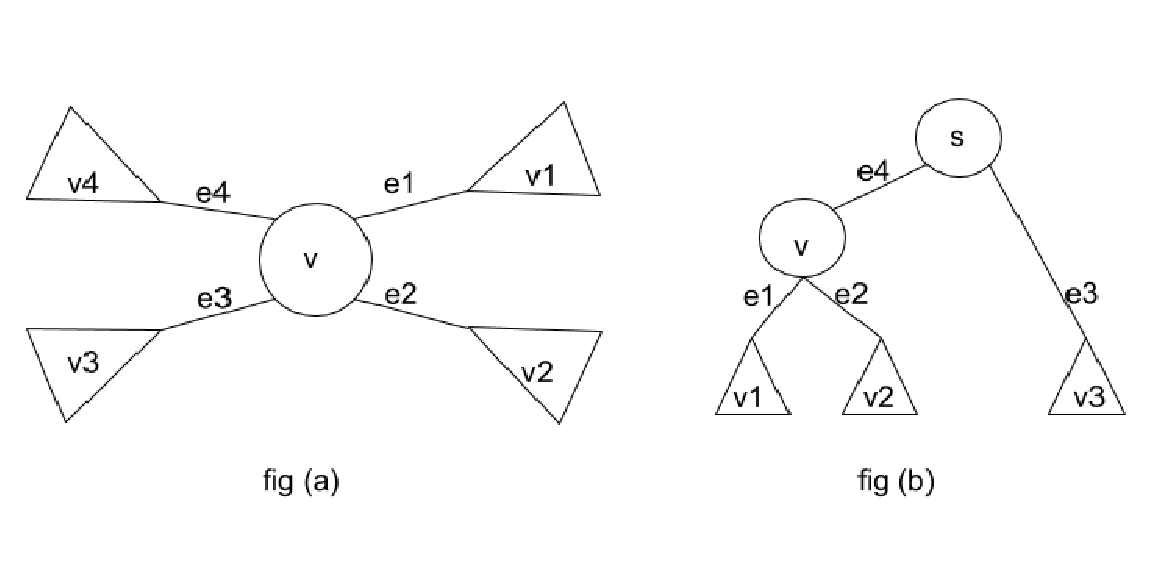
\includegraphics[width=13cm]{images/tree1.eps}
\caption{Reachable vertices of $v$}
\label{fig:lion}
\end{figure}

In figure \ref{fig:lion}(a) a vertex $v$ has four degree with edges as $e1,e2,e3,e4$ and $v1,v2,v3,v4$ corresponds to the number of vertices reachable through those edges respectively. We observed that any vertex from set $v1$ has a shortest path to any vertex in set $v2$ only through $v$. Same is applicable for $v1$ to $v3$, $v4$. Also other paths to be considered are from $v2$ to $v3, v4$ and $v3$ to $v4$.
So $bc[v] = v1*(v2+v3+v4) + v2*(v3*v4) + v3*v4$.

In general we can say that for a vertex $v$ with a degree $d$, $bc[v]$ can be calculated using the equation \ref{eq4} where $v_{i}$ corresponds to number of vertices reachable from $i_{}^{th}$ edge.

\begin{equation} \label{eq4}
bc[v] = \sum_{i=1}^{d-1} v_{i}*(v_{i+1}+..+v_{n})
\end{equation}

Hence for calculating betweenness centrality we need to determine the number of vertices reachable through each edge of that vertex.

The proposed algorithm is divided into two pass.
\vspace{-0.5em}
\begin{enumerate}

  \item Computes the number of reachable vertices for each edge of a vertex.
  \item Computes Betweenness Centrality for a vertex using the values computed in the first pass.
\end{enumerate}
\begin{algorithm}
\caption{Betweenness Centrality of tree}
Select a root vertex $s$ arbitrarily\;
pass1($s$,-1)\;
pass2()\;
\end{algorithm}


\hspace{-1.5em}The proposed algorithm is as follows:
\\
A vertex $s$ is chosen arbitrarily as root. First pass and second pass are then done on the tree considering $s$ as root.

\begin{figure}[htp]
\centering
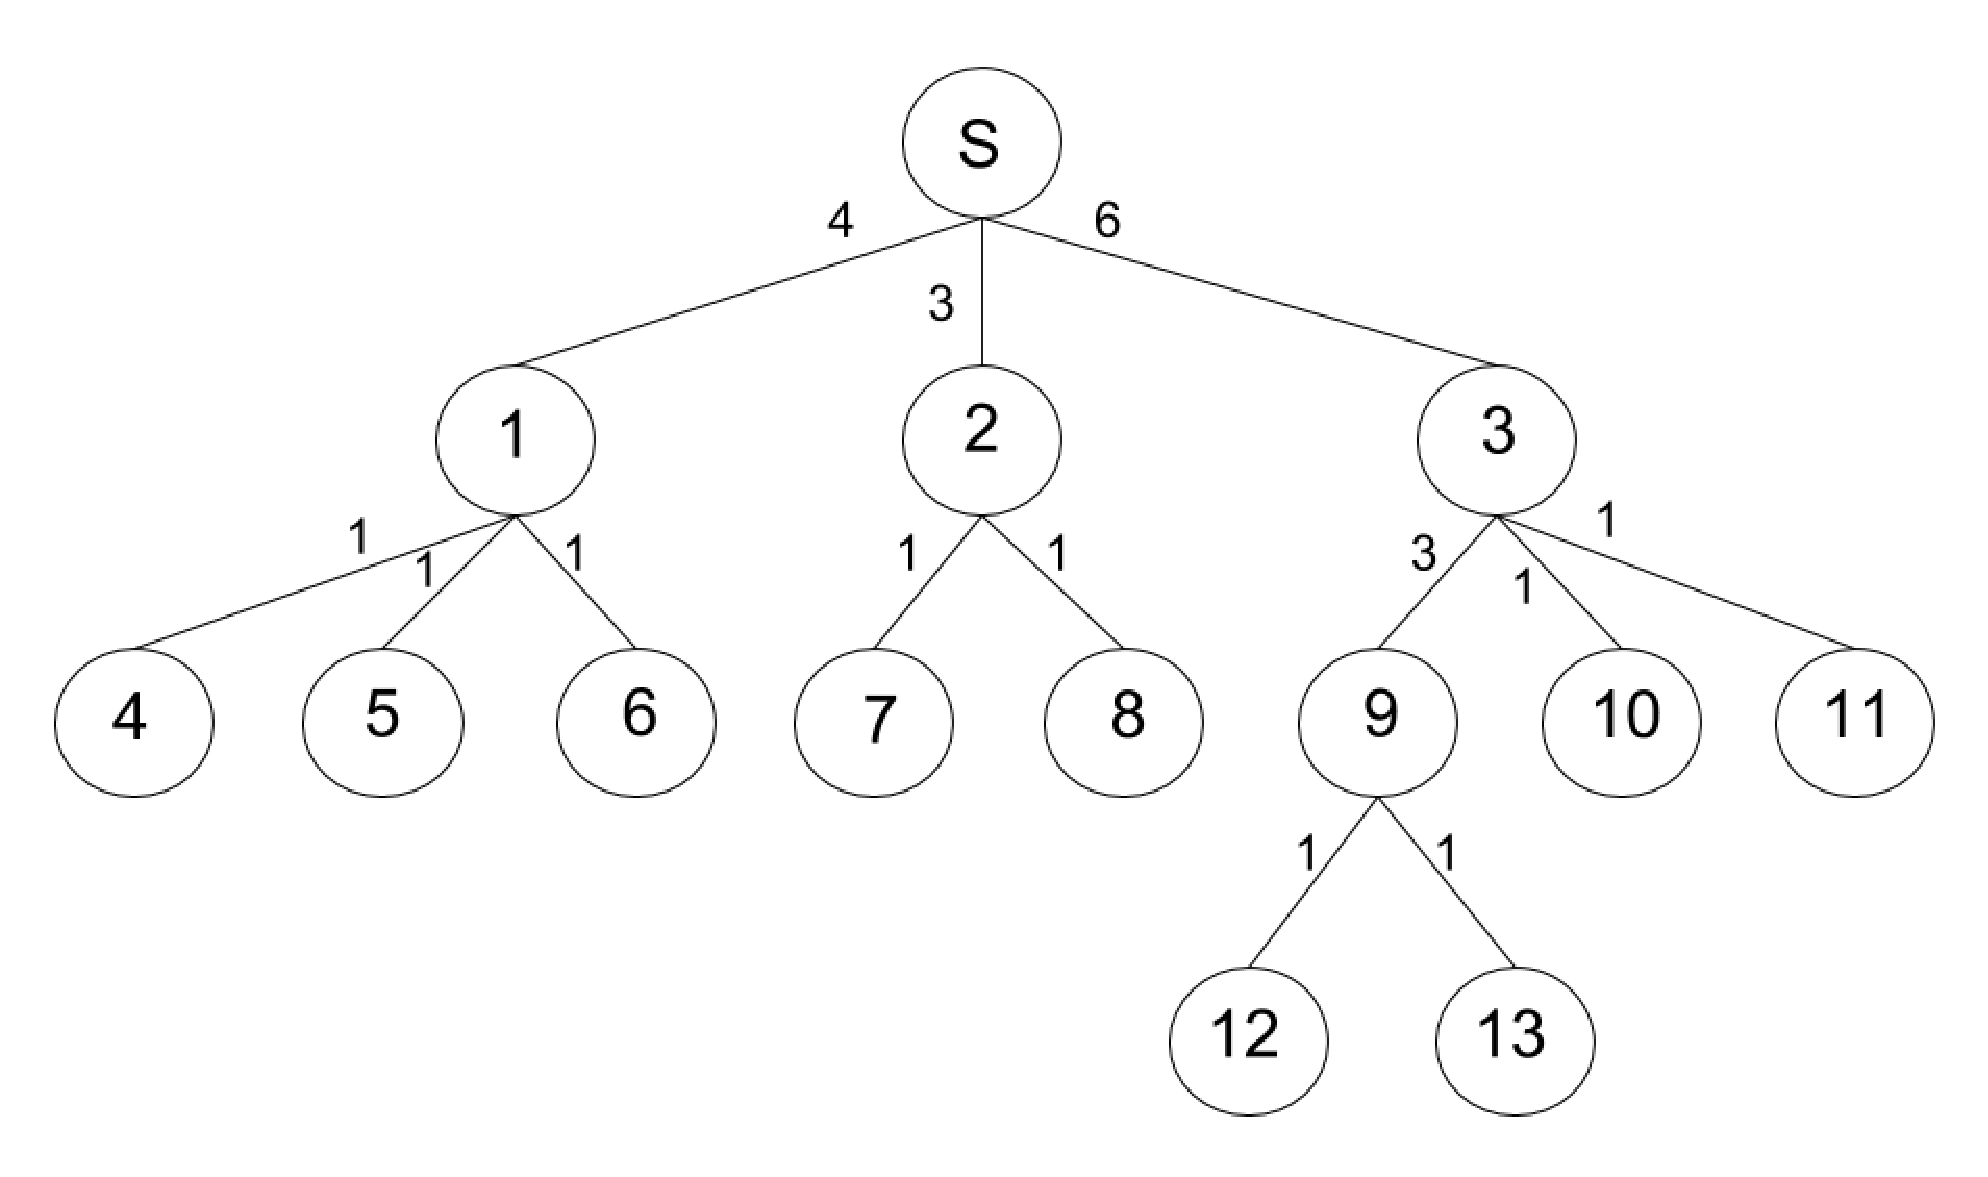
\includegraphics[width=13cm]{images/exampletree.eps}
\caption{Example of Tree}
\label{fig:extree}
\end{figure}

\section{First Pass of Tree Algorithm}
\begin{algorithm}
%\KwResult{Write here the result }
dfs$(child, parent)$ \\
$sum \leftarrow 0$\;

\For{each neighbour vertex $v$ of $child$}{
\If{$v \neq parent$}{
$temp \leftarrow$ dfs($v,child$)\;
$sum \leftarrow sum + temp$\;
Push $temp$ to list[$child$]\;
}
}
return $sum + 1$\;
\caption{Pass1 of Tree Algorithm}

\end{algorithm}
Depth First Search(DFS) is performed on tree starting from $s$. Every vertex $v$ returns the number of vertices in its own subtree including the vertex $v$ to its parent $p$. The parent vertex adds the returned value from all its children to its own list.
Vertex $v$ with a degree $d$ has a list of size $d$.
So at the at end of first pass, the list each vertex except source contains $d-1$ elements and source $s$ contains $d$ elements. The reason is that the source $s$ has no parent while every other vertex has exactly one parent. Hence, we need to add total number of vertices reachable through parent for all vertices except $s$.
For example, in figure \ref{fig:extree} vertex '9' returns a value 3 to its parent '3' and vertex 3 adds to its list. Similarly at the end of pass 1, vertex $S$ has values 4,3,6 in its list whereas vertex '3' has values 3,1,1. 
\vspace{-1.0em}
\section{Second Pass of Tree Algorithm}
\vspace{-1.0em}
So, in the second pass, the number of vertices reachable through parent $s$ of a vertex $v$ are determined.
In fig \ref{fig:lion}(b), we know values of $v1,v2$ but to calculate the number of vertices reachable from parent $s$ that is through edge $e4$, we can use the formula as
\\
no of vertices reachable through parent = total no of vertices - 1 - $(v1 + v2)$

In general we can say that,
\begin{equation} \label{eq5}
v_{d} = n - 1 + \sum_{i=1}^{d-1} list[v_{i}]
\end{equation}
where n is total number of vertices in graph, $v_{d}$ is number of reachable vertices through parent $s$.

For example, in figure \ref{fig:extree}, for vertex '3' its list contains values 3,1,1. So to calculate the number of reachable vertices through its parent, applying formula we get (14 - 1 - (3+1+1)) = 8 

After calculating $v_{d}$, it is added to $list[v]$.
Thus the calculated value 8 is added to list of vertex '3'.
Since we know the total no. of vertices reachable from all edges of a vertex, we can calculate Betweenness Centrality using the equation \ref{eq4}.
\\
Each pass visits each node once and thus the time complexity of the algorithm is $O(n)$.


\section{Proof Of Correctness}

For a tree, all the vertices are connected and have a single path and thus that path needs to be shortest. So the Betweenness Centrality value of a vertex $v$ becomes the total number of paths between any pair $s$ and $t$ passing through $v$, $s \neq t, v\neq t, s\neq v$. Now, such a $<s,t>$ pair whose shortest path passes through $v$, needs to be reachable from different edges of $v$. 

Let us assume that the betweenness centrality values calculated by our proposed algorithm is incorrect. Two cases arise that either our algorithm calculates more value of centrality or it calculates less than the actual value for a vertex $v$.

\begin{enumerate}
\item If our proposed algorithm has calculated more centrality value then for a pair $<s,t>$ whose shortest path does not contain $v$, some values are added to $bc[v]$. But according to Algorithm 2, it does not considers any pair $a,b$ which does not pass through $v$ and thus won't add any value to $bc[v]$.
\item If our proposed algorithm has calculated less centrality value then for a pair $<s,t>$ whose shortest path contains $v$, some values are not added to $bc[v]$. 
\\
Algorithm 2 considers does not considers the vertices reachable from same edge. Since pair $<s,t>$ is not considered, then it should be reachable from $v$ through same edge and thus contradicts the information that $v$ lies on shortest path from $s$ to $t$
\end{enumerate}

Thus, both this cases are not possible which proves that our proposed algorithm is sound and complete.
\chapter{ALGORITHM FOR DAGs}
\label{chap:sup}
 
In this chapter, we propose a new algorithm for Betweenness Centrality specifically for DAGs. 
Consider a Directed Acyclic Graph $G \equiv (V,E)$ where set $V$ contains the vertices and set $E$ contains edges of graph $G$. 
First, we tried to apply the proposed algorithm for tree i.e. Algorithm \ref{treealgofull} on DAGs by making duplicate vertices only if a vertex has two or more parents. Converting DAG into a tree with duplicating vertices and then applying the algorithm for trees was less efficient than the existing Brandes' Algorithm. The reason being, multiple shortest paths exists in DAG from vertex $s$ to $t$ where $s$,  $t \in V$, which was not the case for trees. And even after converting DAG to tree, the merging of vertices to compute the exact values becomes the bottleneck for the computing betweenness centrality and no improvement is achieved in terms of execution time.   

So we proposed another algorithm specifically for DAG, which reduces the execution time with respect to Brandes' Algorithm. The outline of proposed algorithm is given in Algorithm \ref{algo:dagoutline}.
\vspace{1em}
\begin{algorithm}

\caption{Betweenness Centrality of DAG}
\label{algo:dagoutline}
Topological sort and Reverse topological sort\;
Backward Propagation()\;
Forward Propagation()\;
\end{algorithm}

\begin{figure}
\centering
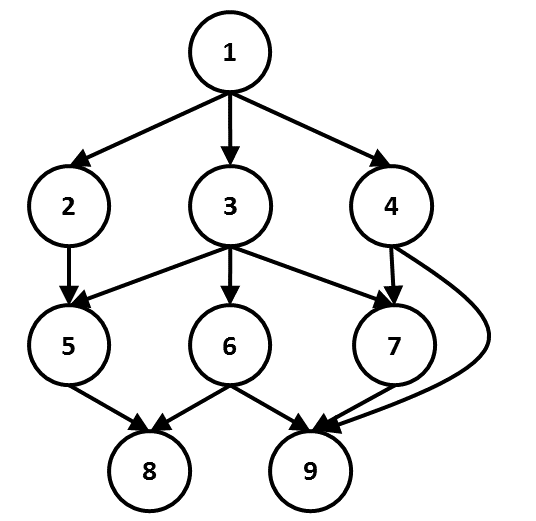
\includegraphics[scale=0.9]{images/Slide3.PNG}
\caption{Example of DAG}
\label{fig:exdag}
\end{figure}

\section{Backward Propagation Phase}
\begin{algorithm}
\caption{Backward Propagation}
\label{backdag}
%\KwResult{Write here the result }
child $\rightarrow v$, parent $\rightarrow p$ \\
\For{each reachable vertex $t$ from $v$}{
\eIf{$d(v,t) + 1 = d(p,t)$}{
$c(p,t) \leftarrow c(p,t) + 1$\;
}
{
\If{$d(p,t) > d(v,t) + 1$ OR $d(p,t) < 0$}{
$d(p,t) \leftarrow d(v,t) + 1$\;
$c(p,t) \leftarrow c(v,t)$\;
}
}
}

\end{algorithm}
As mentioned in Algorithm \ref{algo:dagoutline}, the first step of the proposed algorithm is to compute the topological sort and reverse topological sort of the given graph.

The second step is backward propagation where we use reverse topological sort computed in the first step. The outline of Backward propagation step is given in Algorithm \ref{backdag}. At the end of this step, for any vertex $t$ which is reachable from vertex $v$, the number of shortest paths from $v$ to $t$ and the length of shortest path are stored at vertex $v$. 
For example given in Figure \ref{fig:exdag}, after backward propagation phase, vertex 1, 2, 3, 4 contains information which is described in following table.


% \begin{table}[h!]
% \centering
% \begin{tabular}{|c|c|c|}
% \hline
% vertex & length & count \\
% \hline
% 2 & 1 & 1 \\ 
% \hline
% 3 & 1 & 1 \\ 
% \hline
% 4 & 1 & 1 \\ 
% \hline
% 5 & 2 & 2 \\ 
% \hline
% 6 & 2 & 1 \\ 
% \hline
% 7 & 2 & 2 \\ 
% \hline
% 8 & 3 & 3 \\ 
% \hline
% 9 & 2 & 1 \\ 
% \hline
% \end{tabular}
% \caption{Values stored at Vertex 1}
% \label{tab:data1}
% \end{table}

%     \begin{table}[h!]
%     \centering
%         \begin{tabular}{|c|c|c|}
%             \hline
%             vertex & length & count \\
%             \hline
%             5 & 1 & 1 \\ 
%             \hline
%             8 & 1 & 1 \\ 
%             \hline
%         \end{tabular}
%     \caption{Values stored at Vertex 2}
%     \label{tab:data2}
%     \end{table}


% \begin{table}[h!]
% \centering
% \begin{tabular}{|c|c|c|}
% \hline
% vertex & length & count \\
% \hline
% 5 & 1 & 1 \\ 
% \hline
% 6 & 1 & 1 \\ 
% \hline
% 7 & 1 & 1 \\ 
% \hline
% 8 & 2 & 2 \\ 
% \hline
% 9 & 2 & 2 \\ 
% \hline
% \end{tabular}
% \caption{Values stored at Vertex 3}
% \label{tab:data3}
% \end{table}




% \begin{table}[h!]
% \centering
% \begin{tabular}{|c|c|c|}
% \hline
% vertex & length & count \\
% \hline
% 7 & 1 & 1 \\ 
% \hline
% 9 & 1 & 1 \\ 
% \hline
% \end{tabular}
% \caption{Values stored at Vertex 4}
% \label{tab:data4}
% \end{table}






% \begin{table}
% \centering
% \makebox[0pt]{%
%     \begin{minipage}{0.32\textwidth}
%     \centering
%         \begin{tabular}{|c|c|c|}
%             \hline
%             vertex & length & count \\
%             \hline
%             2 & 1 & 1 \\ 
%             \hline
%             3 & 1 & 1 \\ 
%             \hline
%             4 & 1 & 1 \\ 
%             \hline
%             5 & 2 & 2 \\ 
%             \hline
%             6 & 2 & 1 \\ 
%             \hline
%             7 & 2 & 2 \\ 
%             \hline
%             8 & 3 & 3 \\ 
%             \hline
%             9 & 2 & 1 \\ 
%             \hline
%         \end{tabular}
        
%         \label{tab:vertex1}
%     \end{minipage}
%     %\hfill
%     \begin{minipage}{0.32\textwidth}
%     \centering
%         \begin{tabular}{|c|c|c|}
%             \hline
%             vertex & length & count \\
%             \hline
%             5 & 1 & 1 \\ 
%             \hline
%             6 & 1 & 1 \\ 
%             \hline
%             7 & 1 & 1 \\ 
%             \hline
%             8 & 2 & 2 \\ 
%             \hline
%             9 & 2 & 2 \\ 
%             \hline
%         \end{tabular}
        
%         \label{tab:vertex3}
%     \end{minipage}
%     %\hfill
%     \begin{minipage}{0.32\textwidth}
%     \centering
%         \begin{tabular}{|c|c|c|}
%             \hline
%             vertex & length & count \\
%             \hline
%             5 & 1 & 1 \\ 
%             \hline
%             8 & 1 & 1 \\ 
%             \hline
%         \end{tabular}
        
%         \label{tab:vertex2}
%         \hspace{0.2em}
%         \begin{tabular}{|c|c|c|}
%             \hline
%             vertex & length & count \\
%             \hline
%             7 & 1 & 1 \\ 
%             \hline
%             9 & 1 & 1 \\ 
%             \hline
%         \end{tabular}
        
%         \label{tab:vertex4}
%     \end{minipage}%
% }
% \caption{Values stored at vertices 1-(a), 3-(b), 2-(c), 4-(d)}
% \end{table}





\begin{table}[!htb]
\centering

    \subtable[]{
    \centering
        \begin{tabular}{|c|c|c|}
            \hline
            Reachable vertex & length & count \\
            \hline
            2 & 1 & 1 \\ 
            \hline
            3 & 1 & 1 \\ 
            \hline
            4 & 1 & 1 \\ 
            \hline
            5 & 2 & 2 \\ 
            \hline
            6 & 2 & 1 \\ 
            \hline
            7 & 2 & 2 \\ 
            \hline
            8 & 3 & 3 \\ 
            \hline
            9 & 2 & 1 \\ 
            \hline
        \end{tabular}
        \label{tab:vertex1}
    }
    %\hfill
    \subtable[]{
    \centering
        \begin{tabular}{|c|c|c|}
            \hline
            Reachable vertex & length & count \\
            \hline
            5 & 1 & 1 \\ 
            \hline
            6 & 1 & 1 \\ 
            \hline
            7 & 1 & 1 \\ 
            \hline
            8 & 2 & 2 \\ 
            \hline
            9 & 2 & 2 \\ 
            \hline
        \end{tabular}
        \label{tab:vertex3}
    }
    %\hfill
    \subtable[]{
    \centering
        
        \begin{tabular}{|c|c|c|}
            \hline
            Reachable vertex & length & count \\
            \hline
            5 & 1 & 1 \\ 
            \hline
            8 & 1 & 1 \\ 
            \hline
        \end{tabular}
        \label{tab:vertex2}
        }
         \subtable[]{
        \begin{tabular}{|c|c|c|}
            \hline
            Reachable vertex & length & count \\
            \hline
            7 & 1 & 1 \\ 
            \hline
            9 & 1 & 1 \\ 
            \hline
        \end{tabular}
        \label{tab:vertex4}
    }

\caption{Values stored at vertices 1-(a), 3-(b), 2-(c), 4-(d)}
\end{table}



Table \ref{tab:vertex1} describes the information stored at vertex 1. So, the first tuple 2, 1, 1 implies that vertex 2 is at a shortest distance of length 1 and only 1 such path exists. Whereas tuple 8, 3, 3 implies that vertex 8 is at a shortest distance of length 3 and 3 such path exists. Similarly for other vertices, values get computed and are stored at each vertex.

In reverse topological sort order, any vertex $t$ pushes the information it possess to all its parents. Reverse topological sort order is used because we are pushing information from a child to a parent so the child's information should be computed first and it should not change, otherwise the changed value propagates to the other vertices in case the order is not considered. 

A vertex $u$ updates the values at its parent $w$.
While updating values for vertex $v$ such that shortest path length from $u$ to $v$ is $x$ with count $c1$ then based on values present at vertex $w$ three cases arises:
\begin{enumerate}
\item  $x + 1 >$ path length from $w$ to $v$
\item  $x + 1$ = path length from $w$ to $v$
\item  $x + 1 <$ path length from $w$ to $v$
\end{enumerate}
\vspace{-2.0em}
\subsection{Case 1}
\vspace{-1.0em}
Since a shorter path exists through other vertex, so vertex $u$ doesn't change the values for $v$ at vertex $w$.
For example given in Figure \ref{fig:exdag}, vertex '3' tries to update the value at its parent vertex '1' for vertex '9'. The shortest path length from vertex '3' to vertex '9' is 2. Whereas Vertex '4' has already updated its values at vertex '1'. Hence vertex '1' already contains a shortest path to  vertex '9' of length 2 i.e. 1-4-9. When vertex '3' tries to update value 3 as a path length to vertex '9' at vertex '1', it won't update because there already exists a shorter path through some other vertex and in this case vertex '4'. 

\subsection{Case 2}
Since there exists other paths which are of same length as $w$ to $v$ through other vertices, so $u$ only increments the existing number of paths from vertex $w$ to $v$ by $c1$.
In Figure \ref{fig:exdag}, vertex '3' tries to update the value at its parent vertex '1' for vertex '7'. The shortest path length from vertex '3' to vertex '7' is  '1'. Whereas Vertex '4' has already updated its values at vertex '1'. Hence vertex '1' already contains a shortest path to vertex '7' of length 2 with number of paths as 1, i.e. 1-7-9.
So, vertex '3' increments count of number of paths from vertex '1' to vertex '9' by the number of shortest path from vertex '3' to vertex '9' which is 1. Thus vertex '3' has a shortest path of length 2 and number of such paths are 2.

\subsection{Case 3}
Since the shortest path from vertex $w$ to $v$ doesn't exist or is of length greater than the path through $u$, so $u$ updates the shortest path length as $x + 1$ and also the number of such paths as $c1$.
In Figure \ref{fig:exdag}, vertex '5' updates vertex '3' for vertex '8' as path length 1 and number of such paths as 1 since vertex '3' doesn't have any path to vertex '8' before any updates by vertex '6'. 

After backward propagation phase, any vertex $v$ will have total number of shortest paths to each reachable vertex from $v$ and their path length.
\section{Forward Propagation Phase}

\begin{algorithm}
%\KwResult{Write here the result }
\caption{Forward Propagation}
\label{fordag}
$bc[v] \leftarrow$ 0, $v \in V$\;
\For{each parent $p$ of vertex $v$}{
\For{each reachable vertex $t$ from $v$}{
\If{$d(v,t) + 1 = d(p,t)$}{
$\Delta_{vt} \leftarrow c(v,t)/c(p,t)$\;
$\delta{vt} \leftarrow \delta{vt} + \Delta_{vt}*(1 + \delta{pt})$\;
$bc[v] \leftarrow bc[v] + \Delta_{vt}*(1 + \delta{pt})$\; 
}
}
}

\end{algorithm}

In Algorithm \ref{fordag}, $d(v,t)$ is shortest distance calculated in second step from $v$ to $t$ whereas, $c(v,t)$ is count of shortest path from $v$ to $t$. $\Delta_{vt}$ is ratio of number of shortest paths to $t$ which passes through $v$. 
The third step is to calculate Betweenness Centrality in the topological sorted order of vertices computed in the first step. For each parent $p$ of vertex $v$, we check whether there is shortest path to any node $t$ reachable from $v$ such that distance from $p$ is (distance from $v$ + 1). If such a path exists then we calculate Betweenness Centrality which is given in Algorithm \ref{fordag}. 

\section{Space Complexity}
The algorithm requires storing information at each and every vertex $v$. This information is a tuple of each reachable vertex from vertex $v$, shortest length possible, count of number of shortest path.
So in worst case in DAG, all higher numbered vertices are reachable from lower numbered vertices. This makes $n$ entries in the table stored at each vertex. Since there are $n$ vertices and each uses $n$ memory, so worst case space required be $O(n^2)$. 

\section{Summary}
The betweenness centrality values are calculated correctly with reduced execution time with respect to Brandes' Algorithm.
The issue with this algorithm is that it requires a huge amount of space since we store count and distance for each reachable vertex $t$ from $v$ at vertex $v$.
\chapter{ALGORITHM FOR GRAPHS}
\label{chap:graph}
 
In this chapter we discuss about our proposed algorithm for graphs. 
Given is a Graph $G \equiv (V,E)$ where $V$ is total number of vertices and $E$ is total number of edges.

The drawback of proposed algorithm of DAG was huge memory requirement so it is not feasible to apply the same algorithm for graphs. 
What we observed is that Brandes' algorithm makes a vertex as a source and performs SSSP for each and every vertex. But if we select an order such that we can reuse partial SSSP graph which are same for both the vertices. Such an ordering is possible, if we compute SSSP for vertex $v$ then for any neighbour $u$ of $v$ we can reuse that graph partially, provided that $u$ has not yet been considered for SSSP. Similarly, $u$'s graph can be reused for all its neighbours if they are not considered for SSSP.

For a source $w$, the graph which gets formed while SSSP has edges classified at every vertex as $parent$, $cousins$, $children$.
While performing SSSP, if there is a vertex $v$ at height $h$ and another vertex $u$ at height $h+1$ and there is an edge between $v$ and $u$ then for vertex $v$, vertex $u$ is $child$ and for vertex $u$, vertex $v$ is $parent$.
If there is an edge in original graph between any two vertices and not included in SSSP graph, then they are $cousins$ of each other.
For source $w$, its $parent$ and $cousins$ remains to be empty set.

In figure \ref{fig:exgraph1} vertex 0 is considered as source and in figure \ref{fig:exgraph2}, vertex 1 is considered as source. These graphs are SSSP graph which consists of dotted edges representing $cousins$ and directed edges represent $parent$ to $child$ relation.

\begin{figure}
%\centering
\hspace{-6.5em}
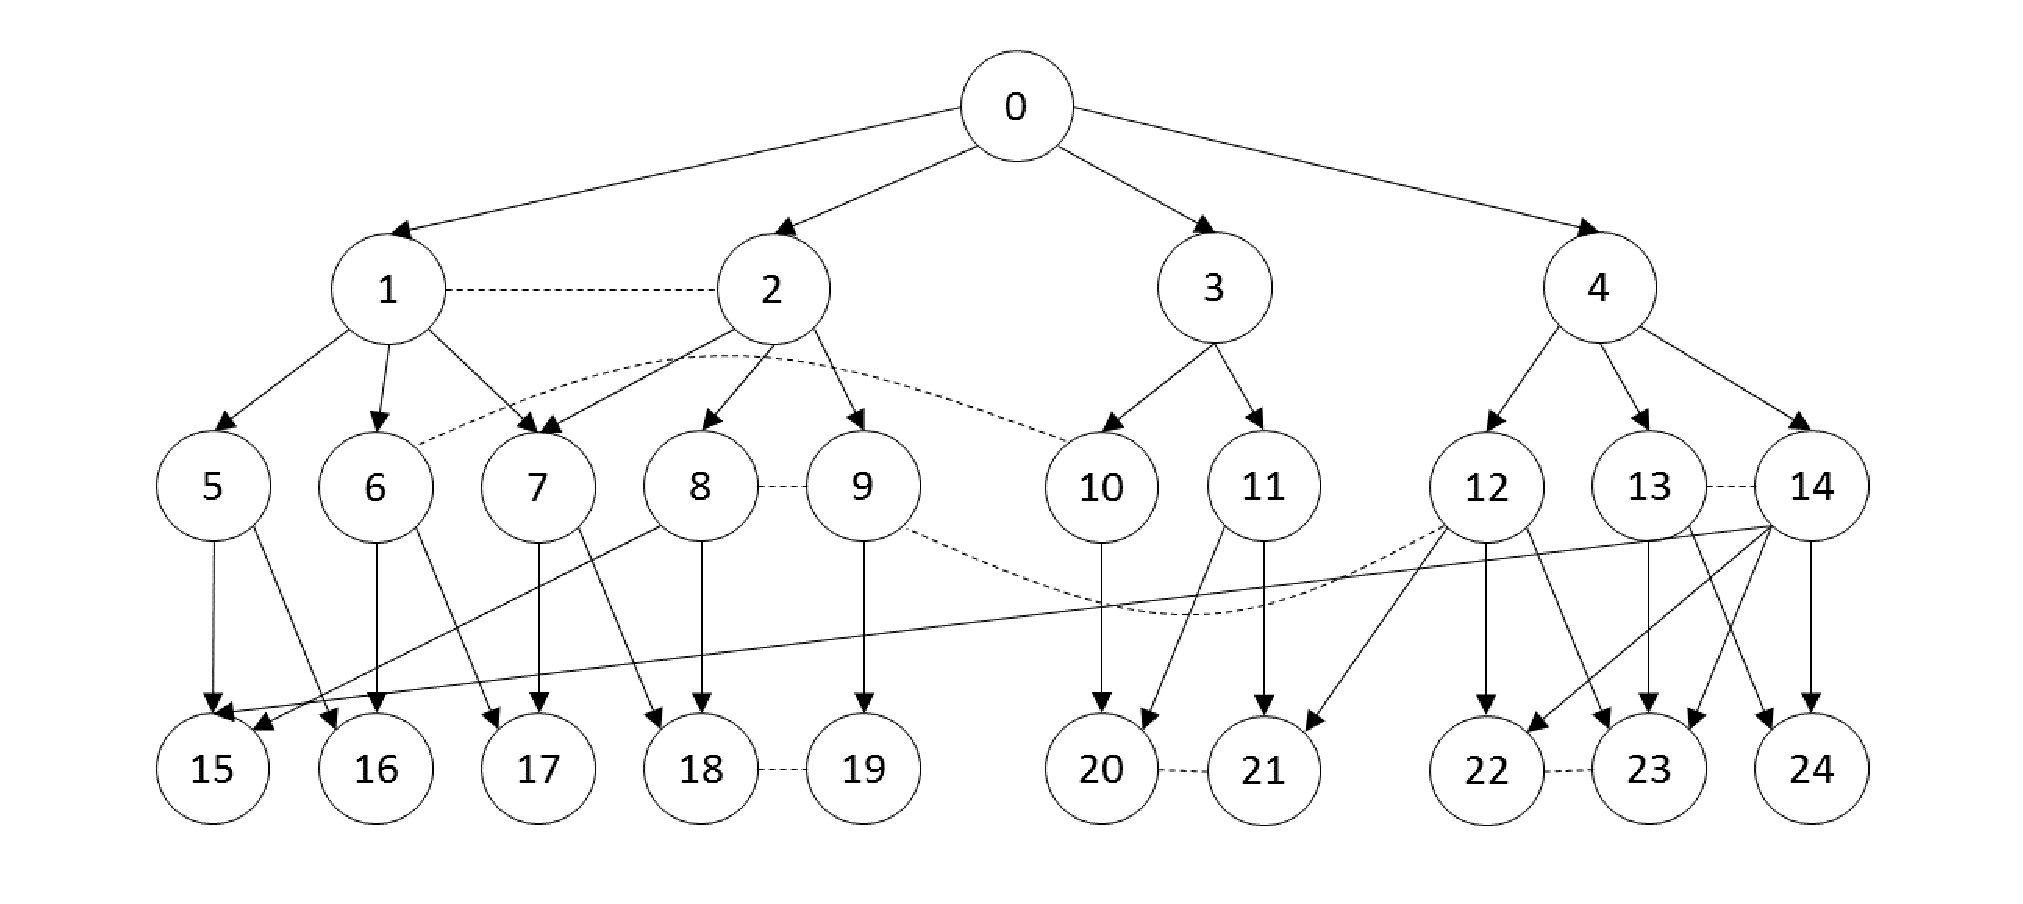
\includegraphics[width=21cm]{images/Slide1.eps}
\caption{SSSP with vertex 0 as source}
\label{fig:exgraph1}
\end{figure}

\begin{figure}
%\centering
\hspace{-6.5em}
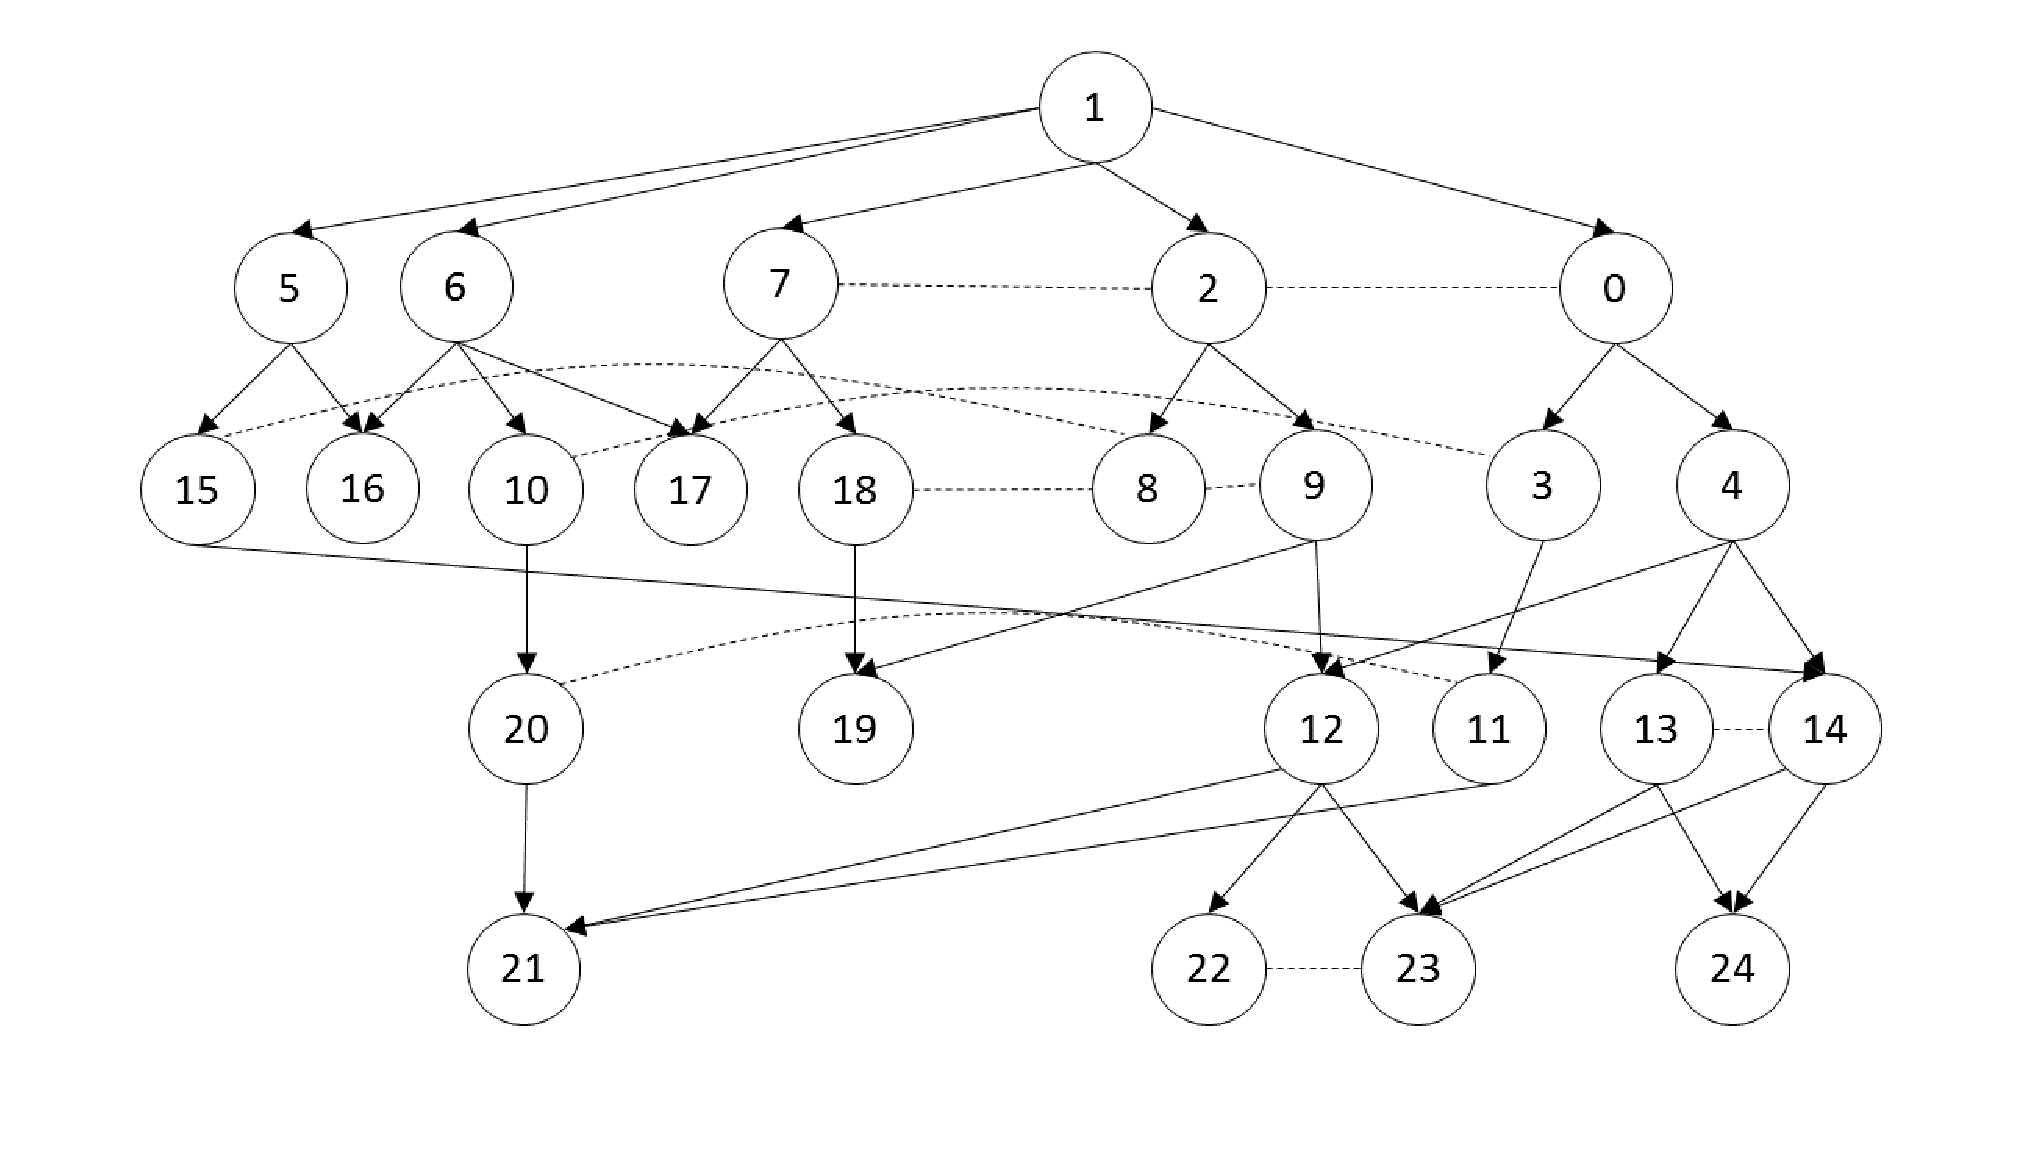
\includegraphics[width=21cm]{images/Slide2.eps}
\caption{SSSP with vertex 1 as source}
\label{fig:exgraph2}
\end{figure}

In figure \ref{fig:exgraph1}, For vertex 6, vertex 1 is a $parent$, vertex 10 is $cousin$ and vertices 16 and 17 are $ children$. Similarly, For vertex 1, vertex 0 is $parent$, vertex 2 is $cousin$ and vertices 5,6 and 7 are $children$. 

For source vertex $w$, $parent$ and $cousin$ remain to be an empty set.
For example, in figure \ref{fig:exgraph1}, vertex 0 has no $parent$ and no $cousin$.
We perform SSSP on vertex 0 and obtain information about each vertex's $parent, children, cousins$. Now we re-use these information to perform SSSP and compute betweenness centrality for vertex 1 which is shown in figure \ref{fig:exgraph2}.

Now to compute SSSP graph of $u$, $u$ becomes the source and its $sub-tree$ in graph of $v$ remains unchanged.
Vertex 1 and all its reachable vertices in original SSSP graph becomes $sub-tree$ which remains un-changed in figure \ref{fig:exgraph2}.

If there are any $cousins$ from $sub-tree$ to outside of $sub-tree$ then they will be $children$ in the new graph. These new relation of $parent$ with their $children$ makes the $children$ to form $extended$ $sub-tree$.
$Cousins$ from $extended$ $sub-tree$ gets changed to their $children$ and thus a new parent child link is formed.
In figure \ref{fig:exgraph2}, vertex 2 becomes $child$ of vertex 1, because vertex 2 was $cousin$ in figure \ref{fig:exgraph1} and vertex 1 belongs to $sub-tree$. Also, vertex 10 becomes $child$ of vertex 6, because vertex 10 was $cousin$ in figure \ref{fig:exgraph1} and vertex 6 belongs to $sub-tree$. This makes vertex 2 and 10 and their reachable vertices which are not included in $sub-tree$ in figure \ref{fig:exgraph1} to be included to $extended$ $sub-tree$. Thus vertices 8, 9, 10, 20 are included in $extended$ $sub-tree$. Also cousins from $extended$ $sub-tree$ not belonging to $sub-tree$ and $extended$ $sub-tree$ becomes their $children$. For example, vertex 12 becomes $child$ of vertex 9 in figure \ref{fig:exgraph2} because vertex 12 is not included in any $sub-tree$. 

Hence, we can construct SSSP graph using for $u$ using SSSP graph for $v$.
$\sigma$ values can be easily calculated while making and breaking the links. Then we apply back propagation phase of Brandes' algorithm to calculate Betweenness Centrality. 

The shortcomings of this algorithm is that it takes up a huge amount of space as we need to store graphs for each vertex. Other reason is due to random access nature of memory requirement, improvement in execution time was not achieved. The time complexity remains same but execution time does not decrease compared to Algorithm \ref{algo:brande}.







\chapter{Experimental Results}
\label{chap:results}

We conducted an experimental evaluation of our algorithms, with two major driving goals in mind: study the behavior of the algorithms presented in this paper and compare it with that of state of art algorithm \ref{algo:brande} in terms of execution time.

\section{Implementation and environment}
We implemented our algorithms and the one presented in algorithm \ref{algo:brande} on IITM's Libra cluster node which has 74GB ram size and using 18GB as maximum heap space. 

\vspace{-1.5em}
\section{Results}
We have compared our algorithm with Brandes' algorithm and we found that there is huge reduction in execution time.
\vspace{-1.0em}
\subsection{Results for Algorithm on Tree}
The trees used for the experimental purposes are synthetic trees made through random functions.
As we can see in table \ref{tab:res1}, that as per increase in the number of vertices of the tree, the time taken by Brandes' algorithm increases to a large extent as compared to proposed algorithm. This proves the basis which we stated to reduction in  time complexity for computing betweenness centrality for trees. 

\begin{table}[h!]
\centering
\begin{tabular}{|c|c|c|}
\hline
No.of vertices & Proposed algorithm on tree & Brandes' algorithm \\
\hline
 & Time in ns & Time in ns\\ 
\hline
2000 & 108175589 & 76791051421 \\ 
\hline
4000 & 110450761 & 387301630614 \\ 
\hline
6000 & 120499273 & 1093484042473 \\ 
\hline
8000 & 134970756 & 2005514757385 \\ 
\hline
\end{tabular}
\caption{Comparison of Brandes' algorithm with our algorithm}
\label{tab:res1}
\end{table}

\subsection{Results for Algorithm on DAGs}
The trees used for the experimental purposes are synthetic trees made through random functions.
As we can see in table \ref{tab:res1}, that as per increase in the number of vertices of the tree, the time taken by Brandes' algorithm increases and the time required by our algorithm increases to a large extent but still is less than Brandes' algorithm. As the number of vertices are increased, not much performance gain is achieved because we use huge memory and once the memory is used up, the program takes huge amount of time swapping the memory in and out of ram. Also for more higher number of vertices, our algorithm doesn't work the heap space provided.
Hence we can conclude that, if given enough memory to compute betweenness centrality, our proposed algorithm beats the Brandes' algorithm.


\begin{table}[h!]
\centering
\begin{tabular}{|c|c|c|c|}
\hline
No.of vertices & No.of edges & Proposed algorithm on DAG & Brandes' algorithm \\
\hline
 & & Time in ns & Time in ns\\ 
\hline
20000 & 91207 & 57927664569 & 120239411956 \\ 
\hline
25000 & 111852 & 88914295841 & 206825800469 \\ 
\hline
27000 & 121079 & 109585676633 & 246413985818 \\ 
\hline
30000 & 134769 & 124939881885 & 285926048584 \\ 
\hline
32000 & 144339 & 141941467652 & 336415443364 \\ 
\hline
36000 & 163172 & 246004717907 & 391164367990 \\ 
\hline
37000 & 165877 & 333386605803 & 429938532146 \\ 
\hline
38000 & 170896 & 435153434414 & 479553177044 \\ 
\hline
40000 & 179765 & 625092042171 & 626296047344 \\ 
\hline
\end{tabular}
\caption{Comparison of Brandes' algorithm with our algorithm}
\label{tab:res1}
\end{table}
\chapter{Related Work on Betweenness Centrality on Graphs}
\label{chap:relwork}

Betweenness centrality was devised as a general measure of centrality way back in 1977. It applies to a wide range of problems in network theory, including problems related to social networks, biology, transport and scientific cooperation. Then in 1994, Douglas R.White et. al generalized the centrality measures for betweenness on undirected graphs to the more general directed case. Then in 2011, Brandes devised an algorithm for calculating betweenness centrality which by far remains the state of art solution. After his work, lots of research has been done in reducing the execution time and also approximating the betweenness centrality. 

One work where M.E. J.Newman relaxes the assumption of betweenness centrality and counts just the number of shortest path was published in 2005 where the centrality was based on the random walks of the graph. M Barthélemy states in his paper that the in general, the BC is increasing with connectivity as a power law of an exponent. 

First work on approximating betweenness centrality was done by David et. al in 2007 where they approximated on basis of an adaptive sampling technique. Robert Geisberger et. al approximated the BC values such that the unimportant nodes also had a good approximation which was not achieved by other work. In 2016 Matteo Riondato proposed approximation techniques where the algorithms are based on random sampling of shortest paths and offer probabilistic guarantees on the quality of the approximation.

Then the work began on approximating as well as running the program on GPUs to parallelize the algorithm. Keshav Pingali et. al in 2013 calculated the exact BC of a graph where they ares able to extract large amounts of parallelism and showed it can be  applied to large graphs. Kamer Kaya et. al computed Betweenness centrality on GPUs and on heterogeneous architectures in 2013 where they showed that heterogeneous computing, i.e., using both architectures at the same time, is a promising solution for betweenness centrality. David A. Bader further increased the speed up in parallel setting and beat the then fastest algorithm and achieved high performance. 

\chapter{CONCLUSION AND FUTURE WORK}
\label{chap:concl}

We have proposed algorithms on trees, DAGs and graphs.
The proposed algorithms on trees improvises time complexity from $\theta$($n^2$) to $\theta$($n$). Whereas the algorithm on DAGs reduces the execution time with respect to Brandes' algorithm. We plan to implement the Brandes' algorithm in parallel and also approximate the values of centrality further reducing the execution time with allowing some loss in precision.

The proposed algorithm for DAG comes with requirement for huge amount of space and thus won't compute for large graphs of size few million vertices and billion edges. The proposed algorithm for graph reuses the partial computed values but fails to improve execution time.
As overall future work in this area is calculating betweenness centrality for a given single vertex only. Brandes' algorithm calculates the values incrementally and will calculate for all the vertices, but it would be challenging to compute without incrementally and directly for a given vertex. Also optimization based on recent GPUs would lead to reducing the execution time.
%%%%%%%%%%%%%%%%%%%%%%%%%%%%%%%%%%%%%%%%%%%%%%%%%%%%%%%%%%%%
% Appendices.
%\appendix
\label{app:class}
\chapter{CLASSIFICATION AND FEATURE EXTRACTION TECHNIQUES USED}
\section{Classification Techniques}
\subsection{Gaussian Mixture Model}
In statistics, a mixture model is a probabilistic model for representing the presence of subpopulations within an overall population. As the name indicates, train data is modeled as a mixture of Gaussian functions. This is basically linear superposition of Gaussians in the form\\
 \begin{equation}
 p(x) = \sum_{k=1}^{K}\pi_{k}N(x|\mu_{k},\Sigma_{k})
 \end{equation}
The biggest advantage of clustering using Gaussian mixture model over traditional clustering method is that each point can be represented more than one cluster. So, it is kind of best way to represent multi modality in a system. Three parameters in Gaussian mixture model, namely $\Sigma$ (covariance), $\mu$ (mean) and $\pi$ (component proportion) are estimated using expectation maximization (EM) method. EM algorithm has applications in a wide variety of tasks and has been used in the context of various machine learning models. The assumption that Gaussian mixture models take is that all the points are identically and independently distributed. So, the log of likelihood of Eqn (1) over all the points is given by
\begin{equation}
ln p(X|\pi, \mu, \Sigma) = \sum_{n=1}^{N}ln \sum_{k=1}^{K}\pi_{k}N(x|\mu_{k},\Sigma_{k})
\end{equation}  
Now the parameters of the model are estimated by maximizing this log likelihood function over an iterative procedure. This is kind of chicken and egg problem where we first input a set of parameters to the model and in return we get an improved set of parameters. This is done until the point of convergence. The initial set of parameters given to the problem are not selected randomly but are generally the output of k-means clustering. A sample mixture of Gaussians can be viewed in figure \ref{fig:gmm}.
\begin{figure}[!htbp]
\centering
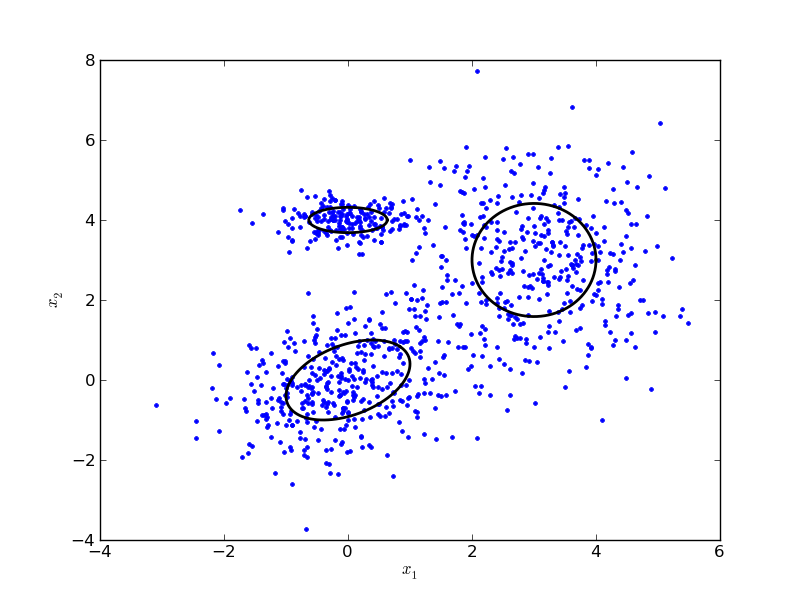
\includegraphics[scale=0.4]{snaps/sample_gmm.png}
\caption{A sample mixture of Gaussians}
\label{fig:gmm}
\end{figure}
\subsection{Hidden Markov Model (HMM)}
Most of the classifiers used in machine learning do not consider the sequence information present in data and they just consider the data as static. The problems that have inherent temporality in them and consists of process that unfolds in time, HMMs have found great use in such problems.\par
The model in HMM is represented by a three-member tuple involving the initial state probabilities, state transition probabilities and observation symbol probabilities. Initial state probabilities define the probability of starting from a particular state. State transition probabilities define the probability of transition from one state to another. Observation probabilities define the probability of observing a symbol from every state.\par
Three major issues of hidden Markov model are:
\begin{itemize}
\item Testing
\item Finding optimal state sequence
\item Training
\end{itemize}
The good news here is that all the three problems are solved and if we have set of observation sequence, then we can define all the three tuples of Hidden Markov Model. We used HTK toolkit for training HMM devised by \cite{HTK}. \par
Two kinds of HMMs used today are Discrete HMMs and continuous density HMMs. In discrete HMMs, observation probabilities in each state are discrete but on the other hand, in continuous density HMM, observation probability is a Gaussian or mixture of Gaussian with its usual parameters.  
\subsection{Support Vector Machine (SVM)}
Support vector machine is one of the most important classifiers in machine learning today. The discussion on support vector machine started after the arrival of perceptron algorithm which focused on obtaining a separating hyperplane between two classes which are linearly separable. But the difference is, Support Vector Machine instead of obtaining just a hyperplane tries to obtain a maximal margin hyperplane. This means that the hyperplane is situated exactly between corner points (also called support vectors) of the two classes. Hyperplane that we need in support vector machine is such that distance of obtained hyperplane from the support vectors of both the classes is maximum from both the classes.  \par
But in a real world, there is hardly any data where the two classes are linearly separable. So, if the data of two classes is overlapping, there is a provision of error in support vector machines. The amount of error tolerance can be specified while training the model. Although in a real world, Support Vector Machines are hardly used in actual data space. This is because of the fact that real world data is not linearly separable. Also as per Cover's theorem, \textit{A pattern recognition problem when cast in higher dimensional space is more likely to be linearly separable than in lower dimensional space.} So, the data is first moved into kernel space which is higher dimensional space or even can be infinite dimensional space. Now in this space, a maximal separating hyperplane is found. Results obtained from support vector machine is highly dependent on parameters given to it. Two of the parameters given to it are kernel width and error tolerance.

\subsection{Random Forest and Decision Trees}
The decision tree is amongst one of the important classifiers in machine learning today. Based on the training data, this algorithm creates a tree where every node from root to leaf gives a decision of which class should the test data belong to. Choice of decision at every node is based on the statistical parameters like variance in the training data. Usually, training time for decision tree is huge, so it is not used when the dataset is large. If we somehow can reduce the size of dataset, then it can be used. \par 
The decision tree is generally not used alone but is used in combination of many. Such a combination of decision trees is known as random forest. Decision given by most number of decision trees is considered to be the final decision.
\section{Feature Extraction}
\subsection{Mel Frequency Cepstral Coefficients (MFCC)}
In sound processing, the mel-frequency cepstrum is a representation of the short-term power spectrum of a sound, based on a linear cosine transform of a log power spectrum on a nonlinear mel scale of frequency.\par
Mel-frequency cepstral coefficients (MFCCs) are coefficients that collectively make up Mel Frequency Cepstrum (MFC). They are derived from a type of cepstral representation of the audio clip which is a nonlinear "spectrum of spectrum". The difference between the cepstrum and the MFC is that in the latter, the frequency bands are equally spaced on the mel scale, which approximates the human auditory system's response more closely than the linearly-spaced frequency bands used in the normal cepstrum. This frequency warping allows for better representation of sound, like in audio compression. MFCCs are commonly derived as follows:
\begin{enumerate} 
\item Take the Fourier transform of (a windowed excerpt of) a signal.
\item Map the powers of the spectrum obtained above onto the mel scale, using triangular overlapping windows.
\item Take the logs of the powers at each of the mel frequencies.
\item Take the discrete cosine transform of the list of mel log powers, as if it were a signal.
\item The MFCCs are the amplitudes of the resulting spectrum.
\end{enumerate}

\subsection{Melody (Pitch)}
Melody extraction is the task of automatically estimating the fundamental frequency corresponding to the pitch of the predominant melodic line of a piece of polyphonic music. Melody extraction is a process of estimating when melody is present and when it is not. It is also a process of estimating correct pitch when the melody is present. The current pitch extraction algorithm used in the work is devised by \cite{justin}.



%%%%%%%%%%%%%%%%%%%%%%%%%%%%%%%%%%%%%%%%%%%%%%%%%%%%%%%%%%%%
% Bibliography.
\nocite{*}
\pagebreak
\begin{singlespace}
  \begin{small}
    \bibliographystyle{unsrt}
	\bibliography{refs}
  \end{small}
\end{singlespace}
%%%%%%%%%%%%%%%%%%%%%%%%%%%%%%%%%%%%%%%%%%%%%%%%%%%%%%%%%%%%
\end{document}
